\part{Multi-Agents Systems and AMAS Theory}

[[NO CHAPTER ??]

As we said at the end of the last part, providing a method able to scale to the needs of the full range of optimization problems would require to it to be capable of adapting itself to the problem at hand.
The main theme of the SMAC team\footnote{\emph{Systèmes Multi-Agents Coopératifs} (Cooperative Multi-Agents Systems)}, in which this thesis has been realized, in the Adaptive Multi-Agent Systems (AMAS) Theory. This theory relates to the design of agent-based complex systems with self-adaptive capabilities.

In this part we will present first a short history of multi-agents systems, before concentrating on the concepts of the AMAS theory.

\section{Multi-Agents Systems}

Multi-Agents Systems (MAS) are a relatively recent field which can be seen as the intersection of Artificial Intelligence (AI) and Systems Theory. As a reminder, the AI field was developed in 1950s as "the science and engineering of making intelligent machines." [[source MacCarthy cf wikipedia]] This rather ambitious project was somewhat toned down during the 70s when the field was the subject of several setbacks leading to an "AI winter"[[REF ? Russell and Norvig ?]], which effects can still be felt today. The commonly accepted reason for this setback was that the researchers have been too much ambitious in their expectations of the breakthroughs which would be produced by the field, and did not take enough in account the inherent complexity of some of the task they were proposing to handle (\emph{e.g. language processing}).

[[TO PUT? Several specific subfield subfields of AI have been defined, among which we can find automated problem solving, machine learning, robotics, knowledge engineering, planning, affective computing \emph{etc.}]]

This disgrace period of the IA field ended with the success of expert systems in the 80s. These systems aim to emulate the ability of a human being to take decisions based on expert knowledge, using inference mechanisms (via an \emph{inference engine}) and a rules database.
However, even expert systems cannot avoid the complexity of modeling knowledge, and are still ultimately limited by the growth of their rules database. This concern, among others (such as privacy of informations) lead to a new field of IA named Distributed Artificial Intelligence (DAI)[[REF?]], where several expert systems collaborate to provide a collective diagnostic of a situation.

In parallel to the developments of AI, another field of knowledge emerged in the beginning of the century, Cybernetics (also called System Theory), the study of self-regulating systems. Interestingly, this field had radically different origins from AI, taking root in social and natural sciences. These two disciplines had a somewhat uneasy coexistence for some times during the 50s, after which AI took the lead and cybernetics[[see on the importance of being emergent - Peter Cariani]].The field knew a revival in the 70s with the "new cybernetics", or "second-order cybernetics", which introduces the study of self-organizing systems and the notion of observer.

It is interesting to note the conflicting nature of AI and cybernetics. AI initially based itself on a reductionist approach of knowledge, using symbol manipulation coming from algebra and logics. Cybernetics was part of the more general [[epistemic/epistemological ??]] upheaval of constructivism.

It is a the conjunction of these two seemingly contradictory fields that was born the study of Multi-Agents Systems.

\subsection{Principles of Multi-Agents Systems}

Before talking about Multi-Agents Systems (MAS), we must explain the notion of \emph{agent}. Several conflicting definitions of what is an agent have been proposed. We keep here the (mostly) consensual one proposed by Wooldridge in \cite{wei1999mutiagent}:

\definition{Agent}{"An \emph{agent} is a computer system that is \emph{situated} in some \emph{environment}, and that is capable of \emph{autonomous action} in this environment in order to meet its design objectives."}

Based on this definition, a MAS is a system composed of several agents, interacting among each other and with their environment.

The \emph{autonomy} of an agent is the fundamental characteristic which differentiates it from, for example, the concept of object. While an object is a passive entity encapsulating some data and functions, waiting to be solicited, an agent is capable of acting and reacting to changes in its environment. From this comparison it should be clear that the concept of agent is, like the concept of object, the building brick of a paradigm which can be used to model a complex reality. And indeed, agents have been used in a great variety of fields, a fact which can contribute to explaining the difficulty to produce an unified definition of the concept.

[[Agent, Environment, Interaction]]

\subsection{Multi-Agents Systems for Distributed Problem Solving}
[[PARLER DE MASCODE]]

In the context of this thesis, we will concentrate on the application of MAS in the specific context of distributed problem solving (DPS). However it can be useful to bear in mind the others possibles application fields: social simulation, biological modeling, systems control, robotics \emph{etc.} and agent-oriented modeling as a programming paradigm in general.

The major part of the literature on the application of MAS to \emph{combinatorial} optimization, mainly in the context of DPS concerns Distributed Constraint Satisfaction Problems (DCSP, or DisCSP) and their extension, Distributed Constrained Optimization Problems (DCOP, or DisCOP).

DCSP is a formalism to model Constraint Satisfactions Problems (CSP) using agents. A CSP is defined as a triplet <$X,D,C$> where:
\begin{compactitem}
\item $X = {x_1, ..., x_n}$ is the set of variables.
\item $D = {D_1, ..., D_n}$ where $D_i$ is the definition domain of $x_i$.
\item $C ={c_1, ..., c_m}$ the set of constraints to satisfy.
\end{compactitem}

The goal is to find an assignment to a set of variables which:
\begin{compactitem}
\item comply with their definition domains.
\item satisfy a set of constraints.
\end{compactitem}

In general, CSP are NP-complete[[REF?]].

Usually, the constraints of a CSP are binary. In this case, the CSP can be represented as a graph for which each vertex is a variable and each constraint an edge.

[[MATH FORMULATION -> GRAPH REPRESENTATION]]

Based from this graph representation the DCSP formalism model a CSP  


In DCOP, the agents try to minimize a global cost function (or alternatively, maximize a global satisfaction) which depends on the states of a set of design variables. Each design variable of the optimization problem is associated to an agent. The agent controls the value which is assigned to the variable.
The global cost function is divided into a set of local cost functions, representing the cost associated with the conjoint state of two specific variables.
An agent is only aware of the cost functions which involve the variable it is responsible for.

[[Put a picture of DCOP]]

While some works successfully used DCOP in the context of continuous optimization\cite{stranders2009decentralised}, this formalism is not adequate to handle the full range of problems considered here. DCOP problems are supposed to be easily decomposable into several cost functions, where the cost values associated to the variables states are supposed to be known. This major assumption does not stand for complex problems (such as MDO problems for example), where the complexity of the models and their interdependencies cause this information to be unavailable in most cases. Trying to model such problems with DCOP would result in a system where most agents are related to every other agent, with unknown cost functions.

[[Change this]]
Moreover, the existing agent-based optimization techniques for DCOP often present similar shortcomings to MDO methods, in the sense that they require a strong expertise to be efficiently applied\cite{Ka2011.6}.

\section{The Adaptive Multi-Agents Systems Theory}

\subsection{Theorem of Functional Adequacy}

The conception of MAS for problem solving is not an easy endeavor. Suffice to observe that most of the multi-agents systems algorithms dedicated to problem solving proposed by the scientific community are nature-inspired (ants, flocks, bees, bats etc.). Indeed, Nature had a long time to experiment on several arduous problem and a lost of subjects at hand. Why would we not take advantage of that? However, such a strategy presents a severe limitation, as it can bring us existing solutions to apply to potential problems, but ultimately cannot help us to find potential solution to some existing problems. By restricting ourself to nature-inspired mechanisms we are bound to their application field.
The inspiration for the internal combustion engine was not found in nature, as no other biological organism than men ever bothered with trying to reach for the Moon\footnote{In total honesty, it is possible that some other organisms already tried to reach for the Moon. But it seems such behavior did not give them enough significant evolutionary advantage to be noteworthy (except of course for a specific cow in the popular nursery rhyme [[put a ref ?]]).}.

In order to overcome this limitation, we need to rely on a more theoretical approach which would help us in the conception of MAS for which we do not know any existing applicable mechanisms. Such an approach is provided by the Adaptive Multi-Agents Systems (AMAS) theory.

The AMAS theory was developed by the SMAC team and formalized in \cite{glize2001adaptation}. It focuses on cooperation as the fundamental mechanism of MAS design.

At the basis of the theory is the modeling of a system as a set of entities, the agents, interacting with each others and with their environment. This modeling is holonic[[?]] at its core, since the agents themselves can also be viewed as systems for which the environment consists of the other agents and the environment of the encompassing system.

The system can be deemed to be \emph{functionally adequate} by an external observer if this latter judges that the system as a whole correctly accomplishes its function in regard of the environment. This external observer can be considered to be a perfect oracle, in a way similar to the Laplace's demon, knowing exactly which will be the consequences of each interactions between the system and its environment\footnote{It is important to understand that, from a theoretical point of view, the notion of functional adequacy is inherently subjective, and depends on the observer. In practice it is however usually more easier to attain a reasonable consensus. For example a natural system will usually be deemed adequate if it survives and thrives in a sustainable way. For an artificial system it is often even easier since the functional adequacy correspond to the function expected by the designer of the system.}.

The AMAS theory identifies three categories of interactions between a system and its environment:
\begin{compactitem}
\item Cooperative action: the acting entity is beneficial to the other.
\item Antinomic action: the acting entity is detrimental to the other.
\item Neutral action: the acting entity has no effect on the other.
\end{compactitem}

From this categorization, the theory draws its formal definition (and fundamental axiom) of functional adequacy:

\definition{Axion of functional adequacy}{A functionally adequate system has no antinomic interaction with its environment}

\begin{figure}
\centering
\subfloat[system not functionally adequate.]{
	\centering
	\begin{minipage}{0.45\textwidth}
		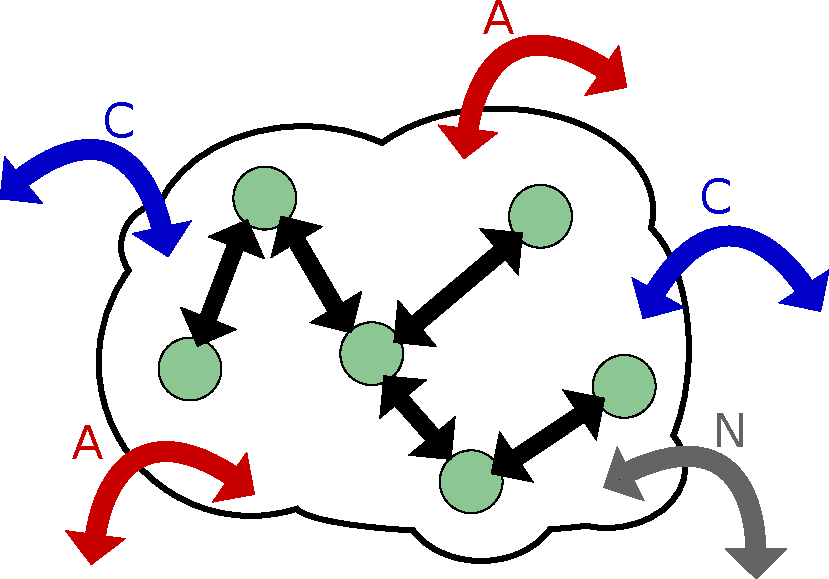
\includegraphics[width=\textwidth]{system_non_adequate}
	\end{minipage}
}
\hfill
\subfloat[functionally adequate system.]{
	\centering
	\begin{minipage}{0.45\textwidth}
		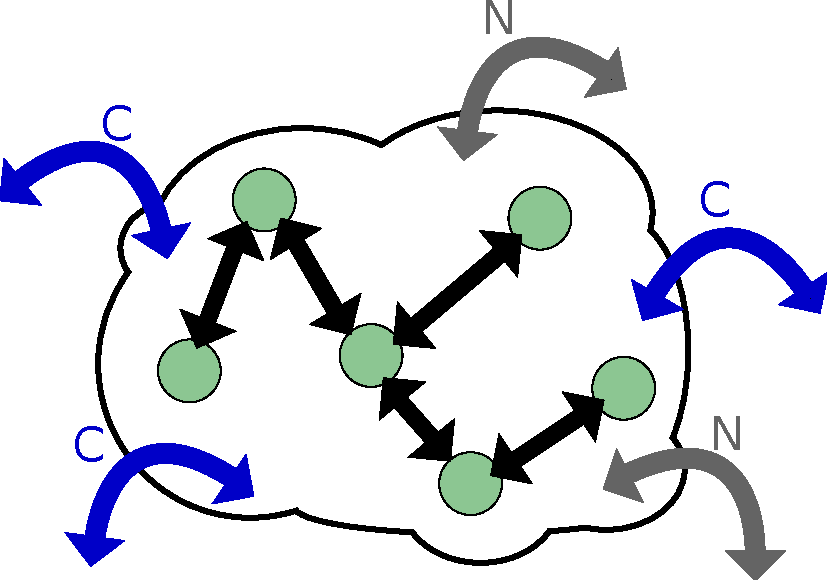
\includegraphics[width=\textwidth]{system_adequate}
	\end{minipage}
}

\caption{Comparison of a system not functionally adequate and a functionally adequate one.}
\label{adequacy_comp}
\end{figure}

An illustration this axiom is shown on \figurename{} \ref{adequacy_comp}.

%\definition{Internal cooperative medium system}{A system in which the agents only have cooperative interactions with each others or their environment[[?]]}

Using this axiom, several properties has been demonstrated concerning a specific set of \emph{internal cooperative medium systems}, defined as systems in which the agents do not have any antinomic or neutral interaction (illustrated on \figurename{} \ref{internal_cooperative_comp}). We will not enter here into the details of these properties and demonstration
, the interested reader can refers to [[REF]]. Suffice to say that these properties lead to the central theorem of functional adequacy:

\definition{Theorem of Functional Adequacy}{For each functionally adequate system there exists a internal cooperative medium system also functionally adequate in the same environment}

\begin{figure}
\centering
\subfloat[system which does not have an internal cooperative medium.]{
	\centering
	\begin{minipage}{0.4\textwidth}
		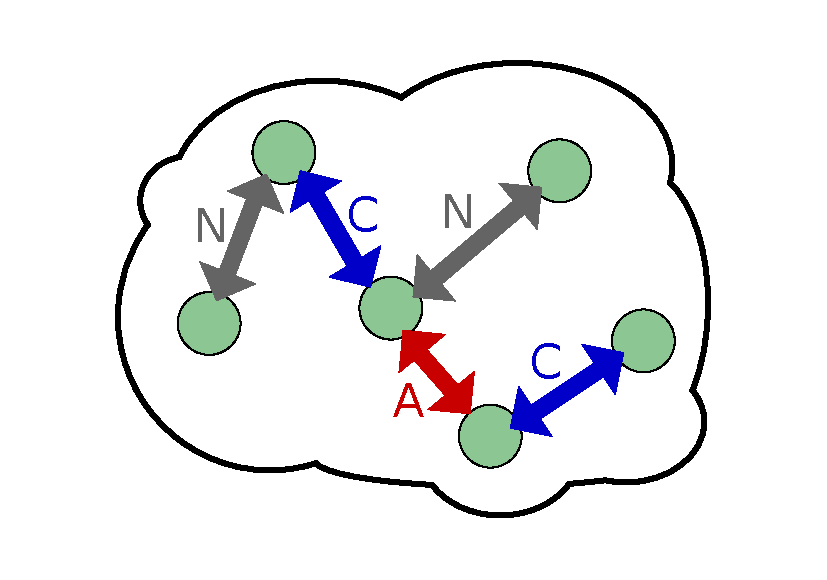
\includegraphics[width=\textwidth]{system_non_cooperative}
	\end{minipage}
}
\hfill
\subfloat[internal cooperative medium system.]{
	\centering
	\begin{minipage}{0.4\textwidth}
		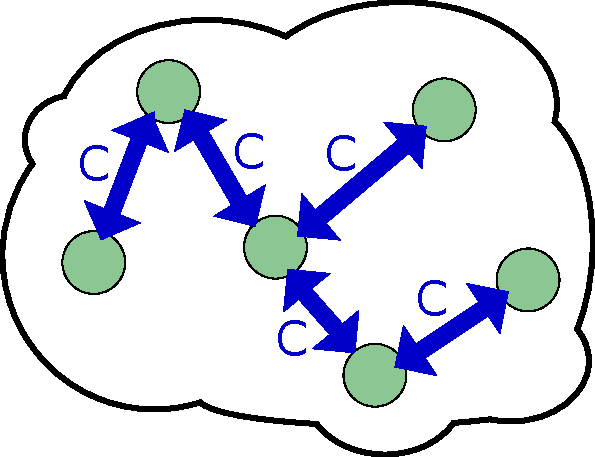
\includegraphics[width=\textwidth]{system_cooperative}
	\end{minipage}
}

\caption{Illustration of internal cooperative medium system.}
\label{internal_cooperative_comp}
\end{figure}

This theorem is at the core of the AMAS approach of system design. We already know that for each problem there is possibly an infinity of equivalent systems producing the same adequate functioning. Using the theorem of functional adequacy we can concentrate on designing an internal cooperative medium system, that is, designing a system were the agents cooperate among themselves and with their environment.

In addition to providing us with a theoretical context, this approach gives us another interesting property: as the design of the system is focused on the local interactions of the agents, we do not need to explicitly take into account the global function of the system. This property is extremely significant. If the global function is complex, it can be extremely difficult to successfully design a system which explicitly tries to achieve the global function (top-down approach). By concentrating on the local functions of the agents, we can spread the complexity and ease the design of the system (bottom-up approach). [[PARLER D'EMERGENCE ? SI OUI QUAND ?]]

\subsection{Cooperative Agents and Non Cooperative Situations}

To guide the designer during the building of such a internal cooperative medium system, the conditions of what make an agent a \emph{cooperative agent} have been further formalized. An agent is said to be cooperative if it satisfies three conditions:
\begin{compactitem}
\item $C_{perception}$ Every perceived signal can be understood without ambiguity
\item $C_{decision}$ Every interpretation must produces useful information
\item $C_{action}$ Every action done based on the decision must be useful
\end{compactitem}

Based on these condition, a set of \emph{Non Cooperative Situations}(NCS) has been identified. These NCS correspond to interactions which are not cooperative and must be removed for the system to be an internal cooperative medium system. The NCS are classified based on the condition they violate. The table in \figurename{} \ref{NCS} shows this classification.

\begin{figure}
\centering
\begin{tabular}{|c|c|}
\hline
\textbf{Violated condition}	& \textbf{Corresponding NCS} \\
\hline
$C_{perception}$     & Incomprehension, Ambiguity     \\
\hline
$C_{decision}$      & Incompetence, Unproductiveness[[?]] \\
\hline
$C_{action}$     & Uselessness, Competition, Conflict\\
\hline
\end{tabular}
\caption{The conditions for cooperation and corresponding NCS}
\label{NCS}
\end{figure}

The different NCS are:

\definition{Incomprehension}{The agent is not able to extract information from a received message.}
\definition{Ambiguity} {The exact meaning of a message cannot be determined, or lacks required informations.}
\definition{Incompetence}{The agent does not have the capabilities to handle a received information.}
\definition{Unproductiveness[[?]]}{A received information does not lead to any useful conclusion.}
\definition{Conflict}{The action of the agent is incompatible with an action from its environment.}
\definition{Competition}{The action of the agent leads to the same result than an action from its environment.}
\definition{Uselessness}{The action of the agent has no effect on itself or its environment.}

A cooperative agent actively tries to avoid these NCS and, should this fail, to solve them to the best of its capabilities. To this end, three distinct mechanisms can be used\cite{bonjean2009engineering}:

\definition{1. Tuning}{The agent can change one or several of its internal parameters (\textit{e.g.}, adjusting the priorities of its behavior rules)}
\definition{2. Reorganization}{The agent can change its relationship with its environment (\textit{e.g.}, removing or creating new links with others agents)}
\definition{3. Evolution}{The agent can change the nature of its environment (\textit{e.g.}, removing or creating new agents)}

The order of these mechanisms usually correspond to their level of disruption (\textit{i.e.}, adjusting its parameters usually has less consequences than creating and removing agents). In general, it is preferable to make the less disruptive possible adjustment. One can for example design the agents based on an escalation principle, where the agents try to solve NCS first by using tuning, escalating to a more disruptive mechanism only when the previous ones failed to solve the NCS. Of course, a NCS situation being by itself disruptive, it is sometime more efficient to immediately make a more radical adjustment in order to solve the NCS more quickly. The designer will have to balance these concerns according to the specificities of the system.

\subsection{The Importance of Locality}
[[Explain how locality is important to scale to big problems and in the concept of emergence => To put in the section A Multi-Agent System for
Optimization ??]]

\subsection{ADELFE - A Method for Designing AMAS} 
[[TODO ? AND MAY ? HERE OR IN THE IMPLEMENTATION PART ?]]